	\subsubsection{UC\theuccount-PR - Gitlab segnala la modifica di una issue al Producer Redmine}
	\begin{figure}[H]
		\centering
		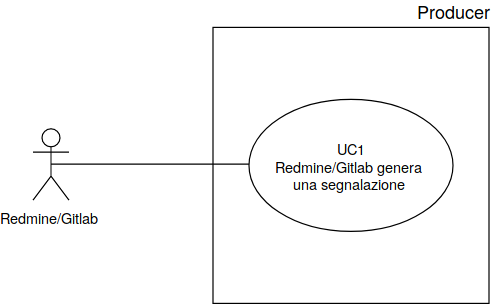
\includegraphics[width=0.7\textwidth]{img/UC1.png}\\
		\caption{UC\theuccount-PR - Redmine segnala la modifica di una issue al Producer Redmine}
	\end{figure}
	\begin{itemize}
		\item \textbf{Codice}: UC\theuccount-PR.
		\item \textbf{Titolo}: Redmine segnala la modifica di una issue al Producer Redmine.
		\item \textbf{Attori primari}: Redmine.
		\item \textbf{Descrizione}: l'invio di una segnalazione avviene
		da parte di Redmine tramite webhook, quando una issue viene modificata.
		\item \textbf{Precondizione}: Viene modificata una issue già aperta su un
		progetto di Redmine e segnalata a \progetto.
		\item \textbf{Postcondizione}: il Producer Redmine riceve la segnalazione da Redmine.
		\item \textbf{Scenario principale}: 
		\begin{enumerate}
			\item Redmine procede all'invio della segnalazione di modifica issue al Producer Redmine.
		\end{enumerate}
		
	\end{itemize}